\begin{figure}[htbp]
\centering
\captionsetup{justification=raggedright,labelsep=none,singlelinecheck=false,labelformat=boldlabel}
\caption[Monthly realized variance of the market and of the factor cross-section]{\footnotesize \textbf{: Monthly realized variance of the market and of the factor cross-section.} The dark line is the value-weighted market portfolio. The band is the 10th to 90th percentile of realized variance across the factors available in each month and the grey line is their median. The vertical scale is logarithmic.}
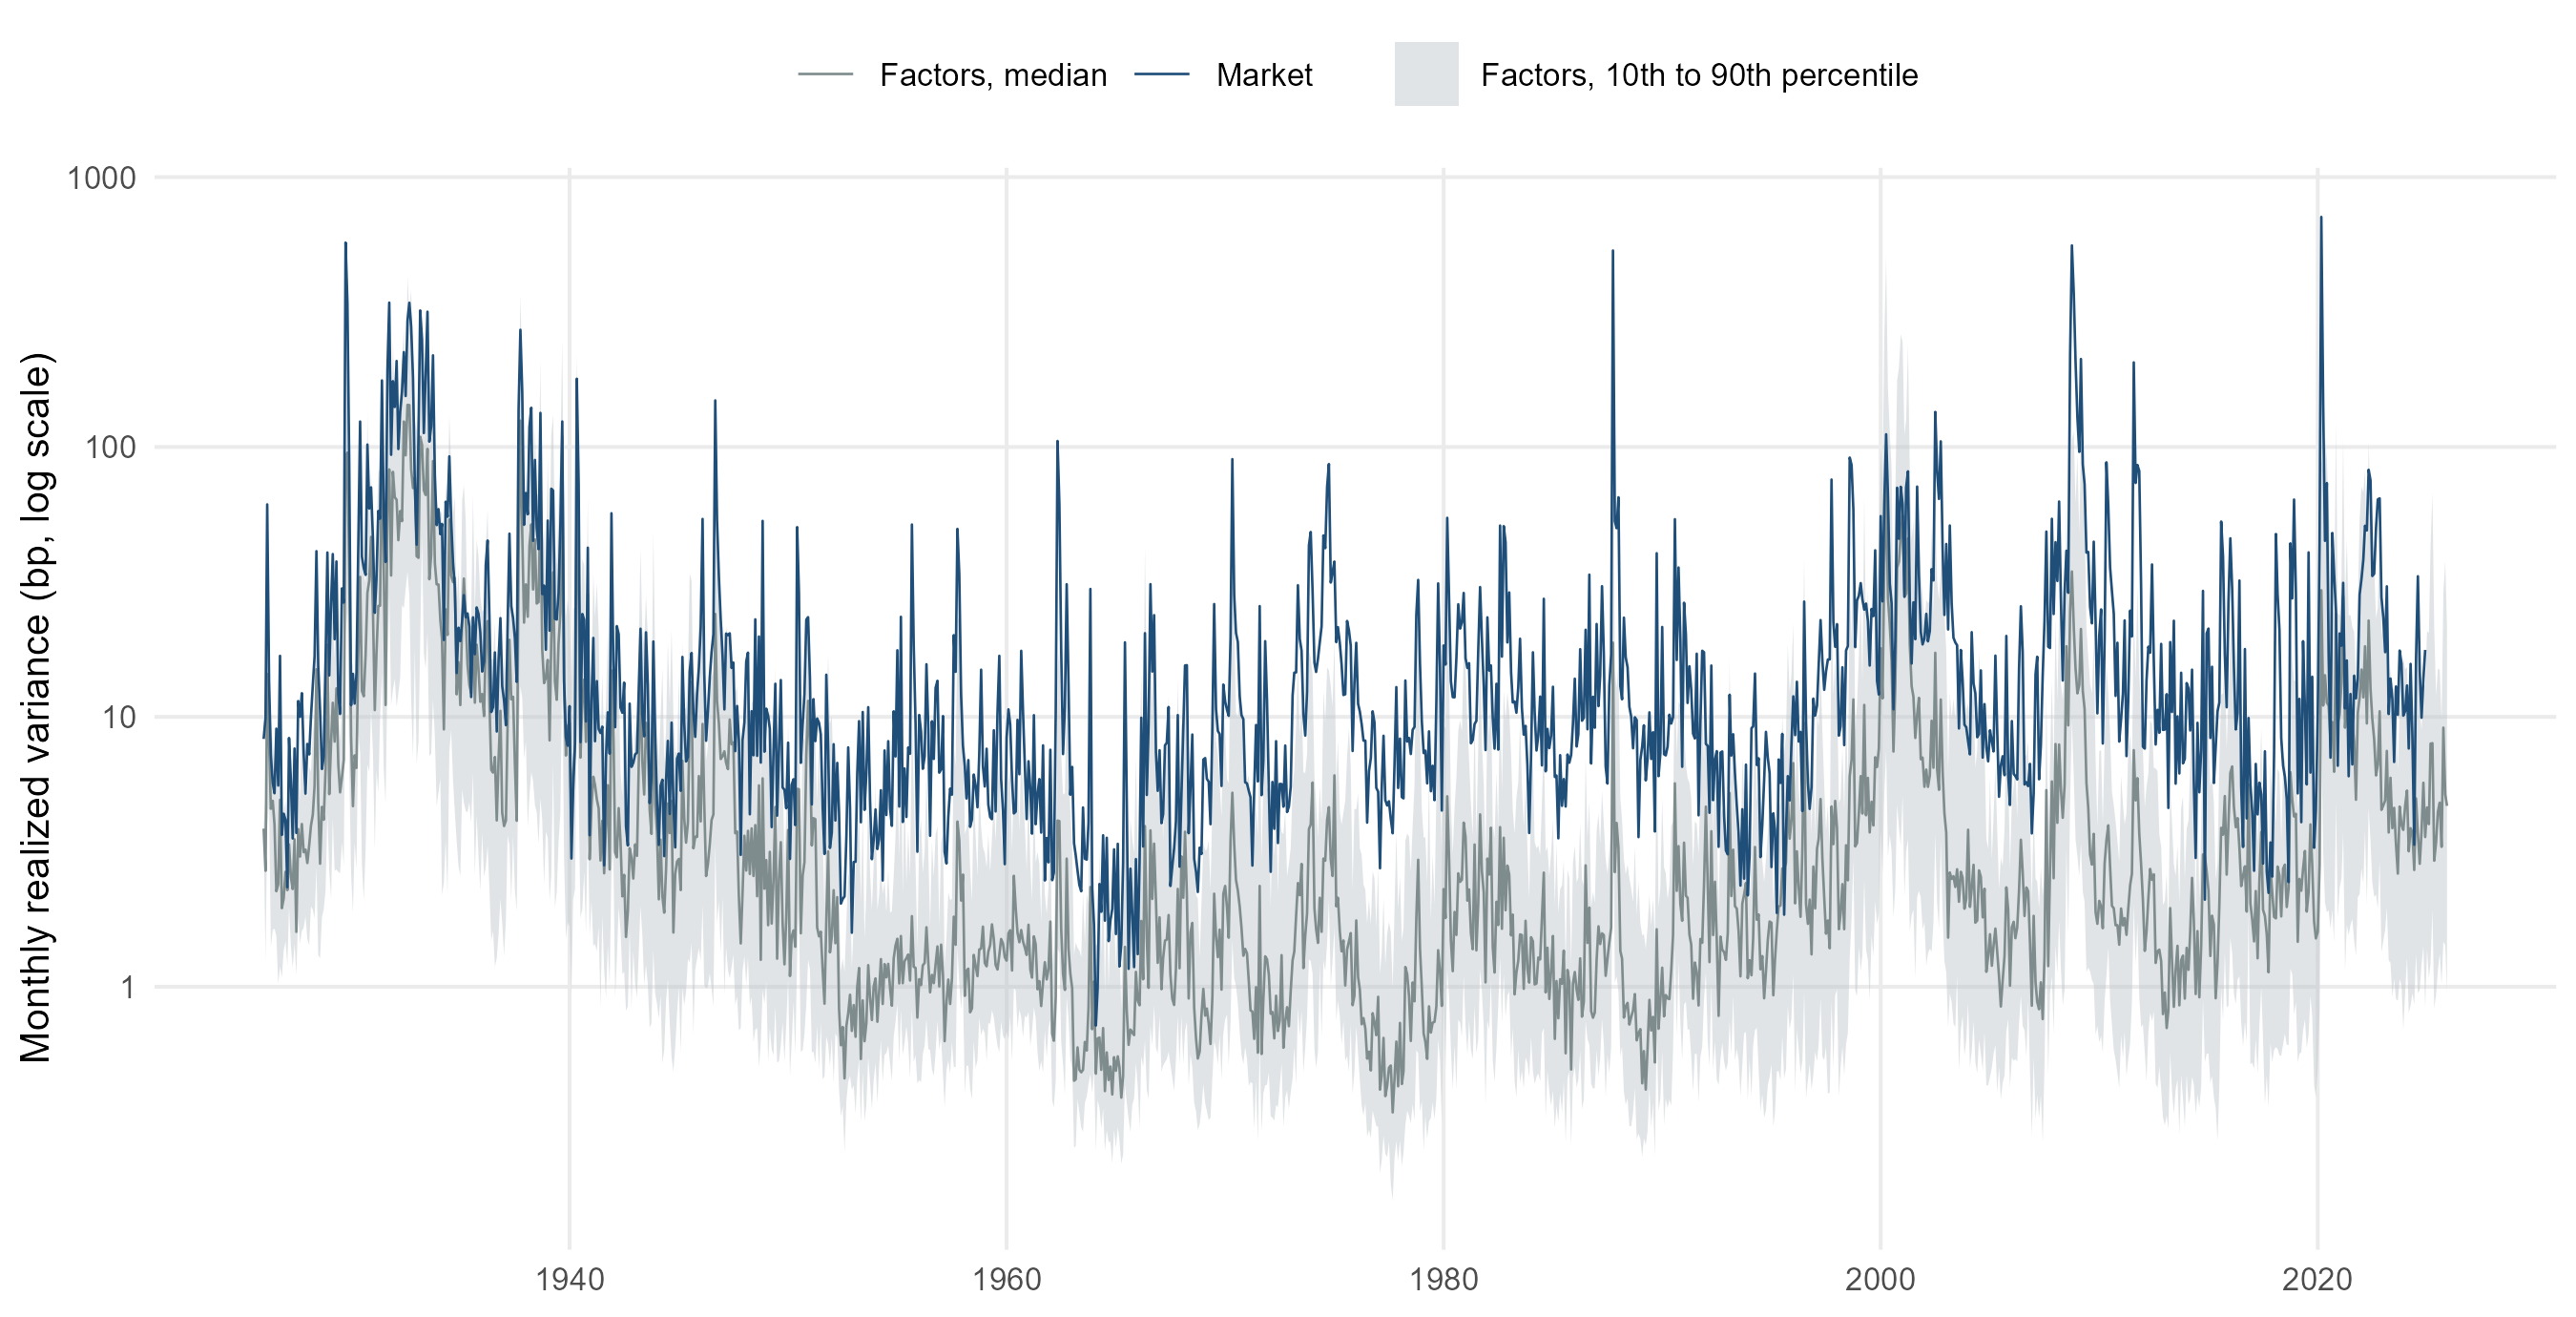
\includegraphics[width=\linewidth]{figures/data_targets.png}
\label{fig:targets}
\end{figure}
